\documentclass[tikz]{standalone}
\usepackage{tikz}
\begin{document}

\tikzset{Karl’s grid/.style={help lines,color=blue!50}}

% 最简单的画十字线,\draw 表示绘制由接下来的命令所描述的路径(path),到分号截止
% 目前来说可以把路径理解为由直线和曲线连接起来的东西,用圆括号里的坐标点描述
% 路径中的点,用一些扩展操作来连接点,最简单的扩展操作就是 -- ,后面必须接上
% 另一个点,表示画一条从前一个点到后一个点的直线
\begin{tikzpicture}
    \draw (-1.5, 0) -- (1.5, 0);
    \draw (0, -1.5) -- (0, 1.5);
    \draw (-3.1, -1.6) -- (-0.1, -1.6) -- (-1.6, -3.1) -- (-1.6, -0.1);
\end{tikzpicture}

% 画曲线,假设起点是x,第一个控制点是y,第二个控制点是w,重点是z
% 绘制出来的曲线将会具有特征:曲线在x处的切线将指向y,在z处的切线将指向z
% 用曲线扩展路径的方式是 .. controls (第一个控制点) and (第二个控制点) .. (重点)
% 去掉y的话,z将把w作为控制点,相当于w做了两次控制点
\begin{tikzpicture}
    % 先画4个灰色填充点
    \filldraw [gray] (0, 0) circle [radius=2pt]
                     (1, 1) circle [radius=2pt]
                     (2, 1) circle [radius=2pt]
                     (2, 0) circle [radius=2pt];
    \draw (0, 0) .. controls (1, 1) and (2, 1) .. (2, 0);
    \draw (5, 5) .. controls (6, 6) .. (7, 5);
\end{tikzpicture}

% 画圆圈
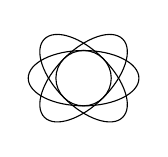
\begin{tikzpicture}
    \draw (0, 0) circle [radius=10pt];
    \draw (0, 0) ellipse [x radius=20pt, y radius=10pt];
    \draw [rotate=45] (0, 0) ellipse [x radius=20pt, y radius=10pt];
    \draw [rotate=-45] (0, 0) ellipse [x radius=20pt, y radius=10pt];
\end{tikzpicture}

% 画矩形
% rectangle将绘制轴对齐,以前后两个点为对角顶点的矩形
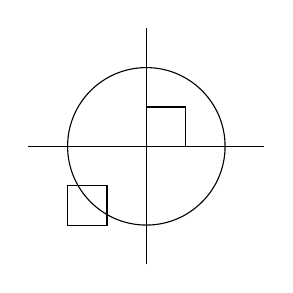
\begin{tikzpicture}
    \draw (-1.5,0) -- (1.5,0);
    \draw (0,-1.5) -- (0,1.5);
    \draw (0,0) circle [radius=1cm];
    \draw (0,0) rectangle (0.5,0.5);
    \draw (-0.5,-0.5) rectangle (-1,-1);
\end{tikzpicture}

% 画网格
% 网格首先和坐标轴重合,然后按照特定的步长绘制,默认步长是1
% 前后顶点只是表明显示由这两个点确定的矩形内的网格,网格线
% 本身并不与矩形的哪个边界重合,而是与坐标轴重合
% 还可以额外指定颜色和线宽,也可以用预先定义的样式
\begin{tikzpicture}
    \draw (0,0) circle [radius=1cm];
    \draw[step=.25cm] (-4.4,-4.4) grid (-1.6,-1.6);
    % \draw[gray, very thin] (-1.5,-1.5) grid (1.5,1.5);
    \draw[Karl’s grid] (-1.5,-1.5) grid (1.5,1.5);
\end{tikzpicture}

% 画圆弧
% arc左边指定路径的起始点,而不是圆弧的圆心,
% 后面指定起始终止角度和圆弧半径
% 相同的命令还可以绘制椭圆,区别在于分别指定x和y方向的半径
% 知道知道起始角度、半径和起点,可以推算出圆心或者椭圆心
% 下面三个弧有相同的起点
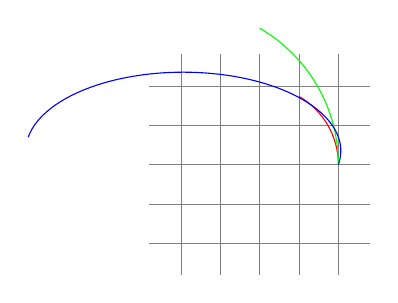
\begin{tikzpicture}
    \draw[step=.5cm,gray,very thin] (-1.4,-1.4) grid (1.4,1.4);
    \draw[red] (10mm, 0mm) arc [start angle=0, end angle=60, radius=10mm];
    \draw[green] (10mm, 0mm) arc [start angle=0, end angle=60, radius=20mm];
    \draw[blue] (10mm, 0mm) arc [start angle=-10, end angle=170, x radius=20mm, y radius=10mm];
\end{tikzpicture}

% 路径裁剪
% 用\clip命令表示接下来所有的路径都只绘制当前矩形内的部分,路径用上一个的
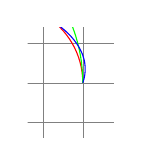
\begin{tikzpicture}
    \clip (3mm, 7mm) rectangle (17mm, -7mm);
    \draw[step=.5cm,gray,very thin] (-1.4,-1.4) grid (1.4,1.4);
    \draw[red] (10mm, 0mm) arc [start angle=0, end angle=60, radius=10mm];
    \draw[green] (10mm, 0mm) arc [start angle=0, end angle=60, radius=20mm];
    \draw[blue] (10mm, 0mm) arc [start angle=-10, end angle=170, x radius=20mm, y radius=10mm];
\end{tikzpicture}
% 还可以在裁剪的同时做绘制,也就是把边界绘制出来
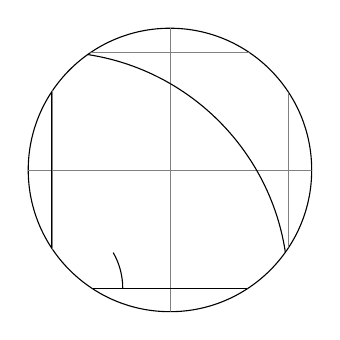
\begin{tikzpicture}[scale=3]
    \clip[draw] (0.5,0.5) circle (.6cm);
    \draw[step=.5cm,gray,very thin] (-1.4,-1.4) grid (1.4,1.4);
    \draw (-1.5,0) -- (1.5,0);
    \draw (0,-1.5) -- (0,1.5);
    \draw (0,0) circle [radius=1cm];
    \draw (3mm,0mm) arc [start angle=0, end angle=30, radius=3mm];
\end{tikzpicture}
% 使用fill来填充路径,和draw不同的用法
% 这里还附带颜色的指定方法20%的绿色和80%的白色做混合
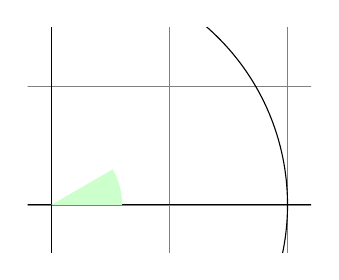
\begin{tikzpicture}[scale=3]
    \clip (-0.1,-0.2) rectangle (1.1,0.75);
    \draw[step=.5cm,gray,very thin] (-1.4,-1.4) grid (1.4,1.4);
    \draw (-1.5,0) -- (1.5,0);
    \draw (0,-1.5) -- (0,1.5);
    \draw (0,0) circle [radius=1cm];
    \fill[green!20!white] (0,0) -- (3mm,0mm) arc [start angle=0, end angle=30, radius=3mm] --cycle;
\end{tikzpicture}

% --cycle参数的示例
% 使用这个参数能让路径自动封闭起来,也就是最后一个点自动连上第一个点
% 下面是几个不一样的用法
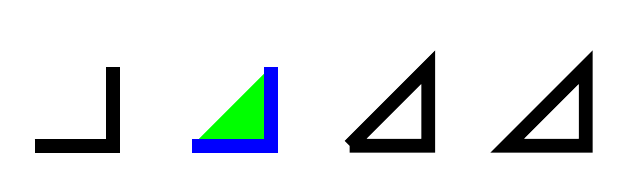
\begin{tikzpicture}[line width=5pt]
    \draw (-2,0) -- (-1,0) -- (-1,1);
    % fill或者filldraw会自动的把路径补成封闭的,但是效果不如 --cycle好看
    \filldraw[fill=green, draw=blue] (0,0) -- (1,0) -- (1,1);
    \draw (2,0) -- (3,0) -- (3,1) -- (2, 0);
    \draw (4,0) -- (5,0) -- (5,1) -- cycle;
    \useasboundingbox (0,1.5); % make bounding box higher
\end{tikzpicture}

% 明暗绘制
% 这个例子还展示了绘制矩形时的一种更方便的方法,指定一个顶点和另一个顶点相对第一个顶点的位移
% 这样就不用计算另一个顶点的坐标了

\begin{tikzpicture}[rounded corners,ultra thick]
    \shade[top color=yellow,bottom color=black] (0,0) rectangle +(2,1);
    \shade[left color=yellow,right color=black] (3,0) rectangle +(2,1);
    \shadedraw[inner color=yellow,outer color=black,draw=yellow] (6,0) rectangle +(2,1);
    \shade[ball color=green] (9,.5) circle (.5cm);
\end{tikzpicture}

% 极坐标的方式表示点位置
% (45:2cm)表示沿45度方向半径为2cm的点
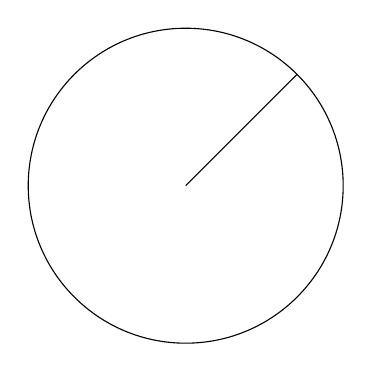
\begin{tikzpicture}
    \draw (0, 0) circle [radius=2cm];
    \draw (0, 0) -- (45:2cm);
\end{tikzpicture}

% +()和++()的使用
% 前者表示添加一个位移,后者表示添加一个位移并且把新的位置作为当前位置
% 二者的区别在于后者会更新当前点,而前者不会,所以前者在指定路径上多个
% 点的时候总是需要指定相对第一个点的位移,而后者由于不断更新当前位置,所以
% 只需要指定相对于最后一个点的位移即可。下面是使用两种方式绘制相同的两个
% 正方形,注意位移的区别。
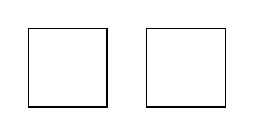
\begin{tikzpicture}
    \def\rectanglepath{-- ++(1cm,0cm) -- ++(0cm,1cm) -- ++(-1cm,0cm) -- cycle}
    \draw (0,0) \rectanglepath;
    \draw (1.5,0) \rectanglepath;
\end{tikzpicture}
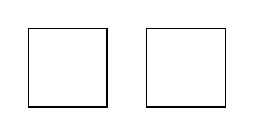
\begin{tikzpicture}
    \def\rectanglepath{-- +(1cm,0cm) -- +(1cm,1cm) -- +(0cm,1cm) -- cycle}
    \draw (0,0) \rectanglepath;
    \draw (1.5,0) \rectanglepath;
\end{tikzpicture}
% 如果在点和++()之间没有 -- 则表示这期间不做绘制,直接把当前点更新到新的位置
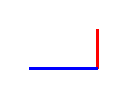
\begin{tikzpicture}
    \draw[red,very thick] (30:1cm) -- +(0,-0.5);
    \draw[blue,very thick] (30:1cm) ++(0,-0.5) -- (0,0);
\end{tikzpicture}
% 绘制箭头
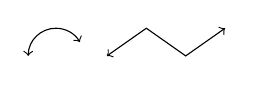
\begin{tikzpicture}
    \draw [<->] (0,0) arc [start angle=180, end angle=30, radius=10pt];
    \draw [<->] (1,0) -- (1.5cm,10pt) -- (2cm,0pt) -- (2.5cm,10pt);
\end{tikzpicture}

% 作用域,在一个作用域内部做设置与外部设置分隔开来互不影响
\begin{tikzpicture}[ultra thick]
    \draw (0,0) -- (0,1);
    \begin{scope}[thin]
    \draw (1,0) -- (1,1);
    \draw (2,0) -- (2,1);
    \end{scope}
    \draw (3,0) -- (3,1);
\end{tikzpicture}

% 坐标系变换xshift之后的点序列都将在这个变换之后的坐标系上绘制,不过这种方式不会更新当前点,
% 所以总是需要相对于原始原点来指定。
\begin{tikzpicture}
    \draw (0, 0) -- (0, 0.5) [xshift=5pt] (0, 0) -- (0, 0.5);
\end{tikzpicture}
% The most useful transformations are xshift and yshift for shifting, shift for shifting to a given point
% as in shift={(1,0)} or shift={+(0,0)} (the braces are necessary so that T E X does not mistake the comma
% for separating options), rotate for rotating by a certain angle (there is also a rotate around for rotating
% around a given point), scale for scaling by a certain factor, xscale and yscale for scaling only in the x-
% or y-direction (xscale=-1 is a flip), and xslant and yslant for slanting. If these transformation and those
% that I have not mentioned are not sufficient, the cm option allows you to apply an arbitrary transformation
% matrix. Karl’s students, by the way, do not know what a transformation matrix is.
% 上面是关于变换的一些命令和功能描述
% 下面是一个在绘制路径过程中修改变换矩阵的例子,(变换顺序待尝试)
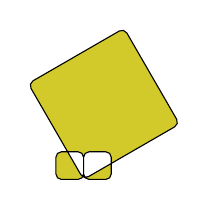
\begin{tikzpicture}[even odd rule,rounded corners=2pt,x=10pt,y=10pt]
    \filldraw[fill=yellow!80!black] (0,0) rectangle (1,1)
    [xshift=10pt,yshift=0pt] (0,0) rectangle (1,1)
    [rotate=30] (0,0) rectangle (4,4);
\end{tikzpicture}

% 循环,基本格式是\foreach <variable> in {<list of values>} <commands>,如果<commands>没有用
% 括号{}括起来,那就把下一个分号之前的所有命令当做<commands>
\begin{tikzpicture}[scale=3]
    \foreach \x in {-1cm,-0.5cm,1cm}
    \draw (\x,-1pt) -- (\x,1pt);
    \foreach \y in {-1cm,-0.5cm,0.5cm,1cm}
    \draw (-1pt,\y) -- (1pt,\y);
\end{tikzpicture}
% 画一行圆圈
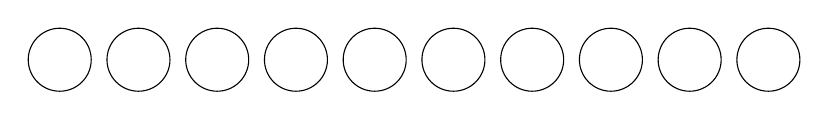
\begin{tikzpicture}
    \foreach \x in {1, ..., 10}
        \draw (\x, 0) circle (0.4cm);
\end{tikzpicture}
% 如果在...之前用了两个数字,那么这两个数字的差就作为循环步长
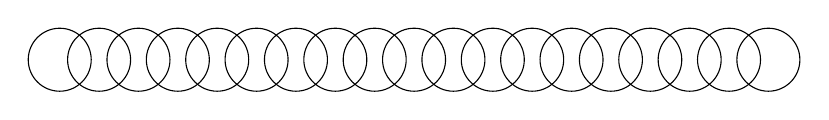
\begin{tikzpicture}
    \foreach \x in {1, 1.5, ..., 10}
        \draw (\x, 0) circle (0.4cm);
\end{tikzpicture}
% 还可以嵌套循环,以及两组分段循环组合在一起,下面的例子都包含了
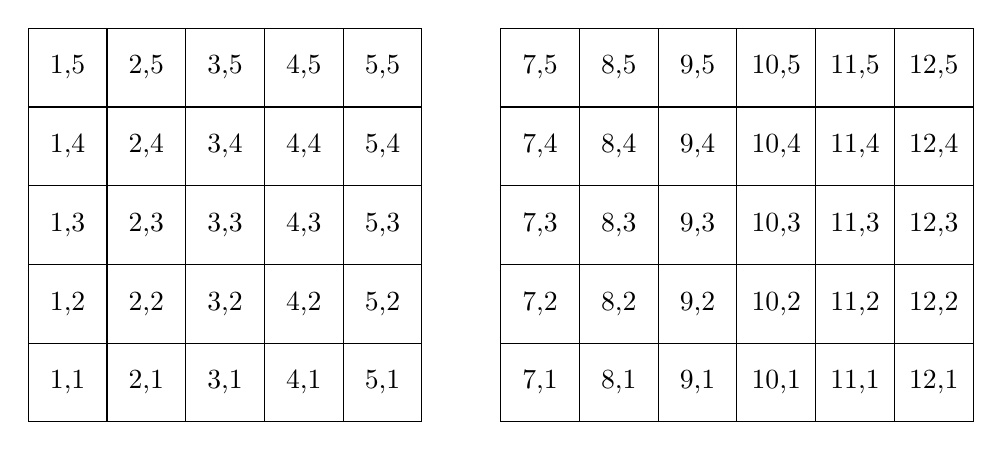
\begin{tikzpicture}
    \foreach \x in {1,2,...,5,7,8,...,12} % 分段的循环组合在一起
        \foreach \y in {1,...,5} % 嵌套内循环
        {
            \draw (\x,\y) +(-.5,-.5) rectangle ++(.5,.5);
            \draw (\x,\y) node{\x,\y};
        }
\end{tikzpicture}

% 添加文本
% 在绘制路径的过程中添加 node 命令,node后接方括号括起来的属性描述和大括号括起来的文字
% 文字的位置就在 node 前面的坐标位置
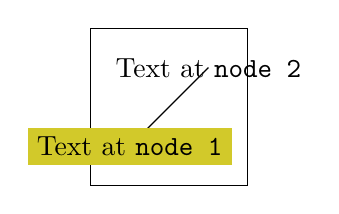
\begin{tikzpicture}
    \draw (0,0) rectangle (2,2);
    \draw (0.5,0.5) node [fill=yellow!80!black]{Text at \verb!node 1!}
            -- (1.5,1.5) node {Text at \verb!node 2!};
\end{tikzpicture}
% 还可以指定node的锚点(south, north, east, west),指定之后,锚点会和坐标位置对齐
% 注意:这里不是说node位于坐标的哪个方位,而是node的东南西北中部位作为
% 锚点和坐标对齐。当把node的north指定为锚点后,整个node是在坐标的南边的。
% 可以多个方向组合
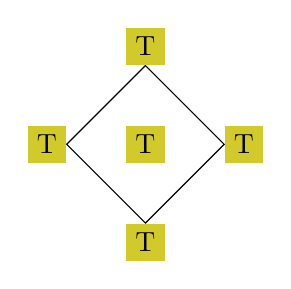
\begin{tikzpicture}
    \draw (0,0) node [fill=yellow!80!black]{T};
    \draw (0,1) node[anchor=south] [fill=yellow!80!black]{T}
    -- (1,0) node[anchor=west] [fill=yellow!80!black]{T}
    -- (0,-1) node[anchor=north] [fill=yellow!80!black]{T}
    -- (-1,0) node[anchor=east] [fill=yellow!80!black]{T} --cycle;
\end{tikzpicture}
% 指定锚点的方式有点反直觉,因此tizk也提供了另外一种指定方式
% 就是说明node位于坐标的哪个方位(above, below, right, left),
% 更进一步,这种方式还可以提供各个方位的位移。
% 可以多个方向组合
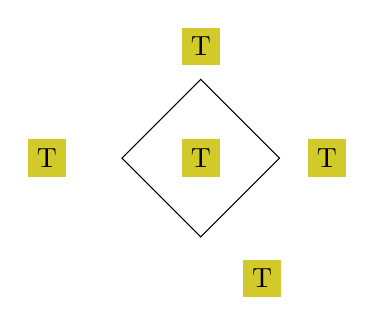
\begin{tikzpicture}
    \draw (0,0) node [fill=yellow!80!black]{T};
    \draw (0,1) node[above=5pt] [fill=yellow!80!black]{T}
    -- (1,0) node[right=10pt] [fill=yellow!80!black]{T}
    -- (0,-1) node[below=15pt, right=15pt] [fill=yellow!80!black]{T}
    -- (-1,0) node[left=20pt] [fill=yellow!80!black]{T} --cycle;
\end{tikzpicture}

% 另一个例子
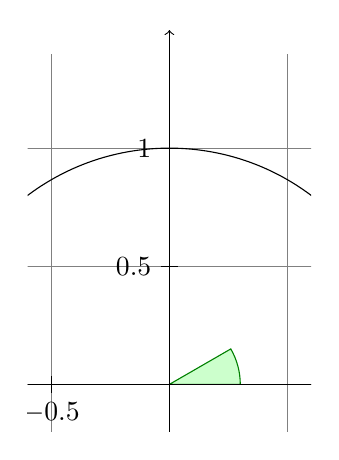
\begin{tikzpicture}[scale=3]
    \clip (-0.6,-0.2) rectangle (0.6,1.51);
    \draw[step=.5cm,help lines] (-1.4,-1.4) grid (1.4,1.4);
    \filldraw[fill=green!20,draw=green!50!black] (0,0) -- (3mm,0mm)
    arc [start angle=0, end angle=30, radius=3mm] -- cycle;
    \draw[->] (-1.5,0) -- (1.5,0); \draw[->] (0,-1.5) -- (0,1.5);
    \draw (0,0) circle [radius=1cm];
    \foreach \x in {-1,-0.5,1}
    \draw (\x cm,1pt) -- (\x cm,-1pt) node[anchor=north] {$\x$};
    \foreach \y in {-1,-0.5,0.5,1}
    \draw (1pt,\y cm) -- (-1pt,\y cm) node[anchor=east] {$\y$};
\end{tikzpicture}
% 在上面的例子中,使用循环变量既作为数值描述了坐标位置,又作为文字显示出来
% 有时希望能显示数学表达式而不是数值,比如0.5想显示成\frac{1}{2},更有甚者,
% 可能想显示\Pi,对于这类数学表达式,tikz并不能理解其含义,这些表达式不能作为
% 数值来描述坐标,只能作为文本显示出来,因此需要同时能描述位置的数值和对应的文本,
% foreach支持二元组形式的循环变量,\v1 / \v2,用斜线分隔,与此同时,
% 循环列表中元素也需要是\v1 / \v2的形式,在循环过程中列表中的二元组会对应的赋值给
% 循环变量二元组,如果列表中某个元素只有一个值,那这个值既当做\v1用也当做\v2用。
% 在下面的例子中就是一个变量放数值,一个变量放文本
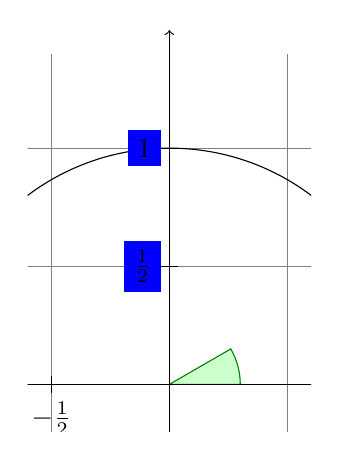
\begin{tikzpicture}[scale=3]
    \clip (-0.6,-0.2) rectangle (0.6,1.51);
    \draw[step=.5cm,help lines] (-1.4,-1.4) grid (1.4,1.4);
    \filldraw[fill=green!20,draw=green!50!black] (0,0) -- (3mm,0mm)
    arc [start angle=0, end angle=30, radius=3mm] -- cycle;
    \draw[->] (-1.5,0) -- (1.5,0); \draw[->] (0,-1.5) -- (0,1.5);
    \draw (0,0) circle [radius=1cm];
    \foreach \x/\xtext in {-1, -0.5/-\frac{1}{2}, 1}
    \draw (\x cm,1pt) -- (\x cm,-1pt) node[anchor=north] {$\xtext$};
    \foreach \y/\ytext in {-1, -0.5/-\frac{1}{2}, 0.5/\frac{1}{2}, 1}
    \draw (1pt,\y cm) -- (-1pt,\y cm) node[anchor=east, fill=blue] {$\ytext$};
\end{tikzpicture}
% 除了把node接在坐标位置后之外,还能把node放在--线和坐标位置之间,表示node
% 将被绘制在线中间,sloped表示让文字贴着线
\begin{tikzpicture}
    \draw (0, 0) -- node[sloped]{in the middle of the line} (5, 5);
\end{tikzpicture}
% 另外一个线上文字的例子,这里是把node放在了..和坐标位置之间,道理一样的
% 除此之外还有一些文字在线上的位置属性设置
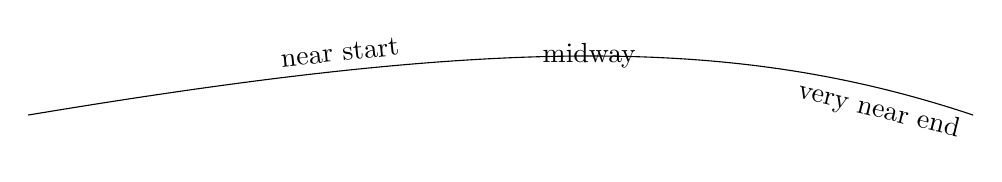
\begin{tikzpicture}
    \draw (0,0) .. controls (6,1) and (9,1) ..
    node[near start,sloped,above] {near start}
    node {midway}
    node[very near end,sloped,below] {very near end} (12,0);
\end{tikzpicture}

% pic 可以理解为预定义的子图形,可以像node一样可以插入
% 具体语法待补充

\end{document}